Due to the high production cross section associated with processes involving the
strong interaction, the monojet signature is a favored experimental signature in
the search for large extra dimensions in the \gls{add} scenario. In the previous
version of this analysis with the ATLAS detector~\cite{MonoJetPaper}, upper
limits on the effective Planck scale $\md$ have been set. Values of $\md$ up to
6.6 and 4.3~TeV for n = 2 and 6 dimensions respectively have been
excluded. \cref{fig:add_2015} shows the expected and observed limits on $\md$ as
a function of the number of extra dimensions in the \gls{add} scenario carried
out in the 3.2~$\ifb$ collected by the \gls{atlas} detector in
2015~\cite{MonoJetPaper}.
\begin{figure}[!h]
  \centering
  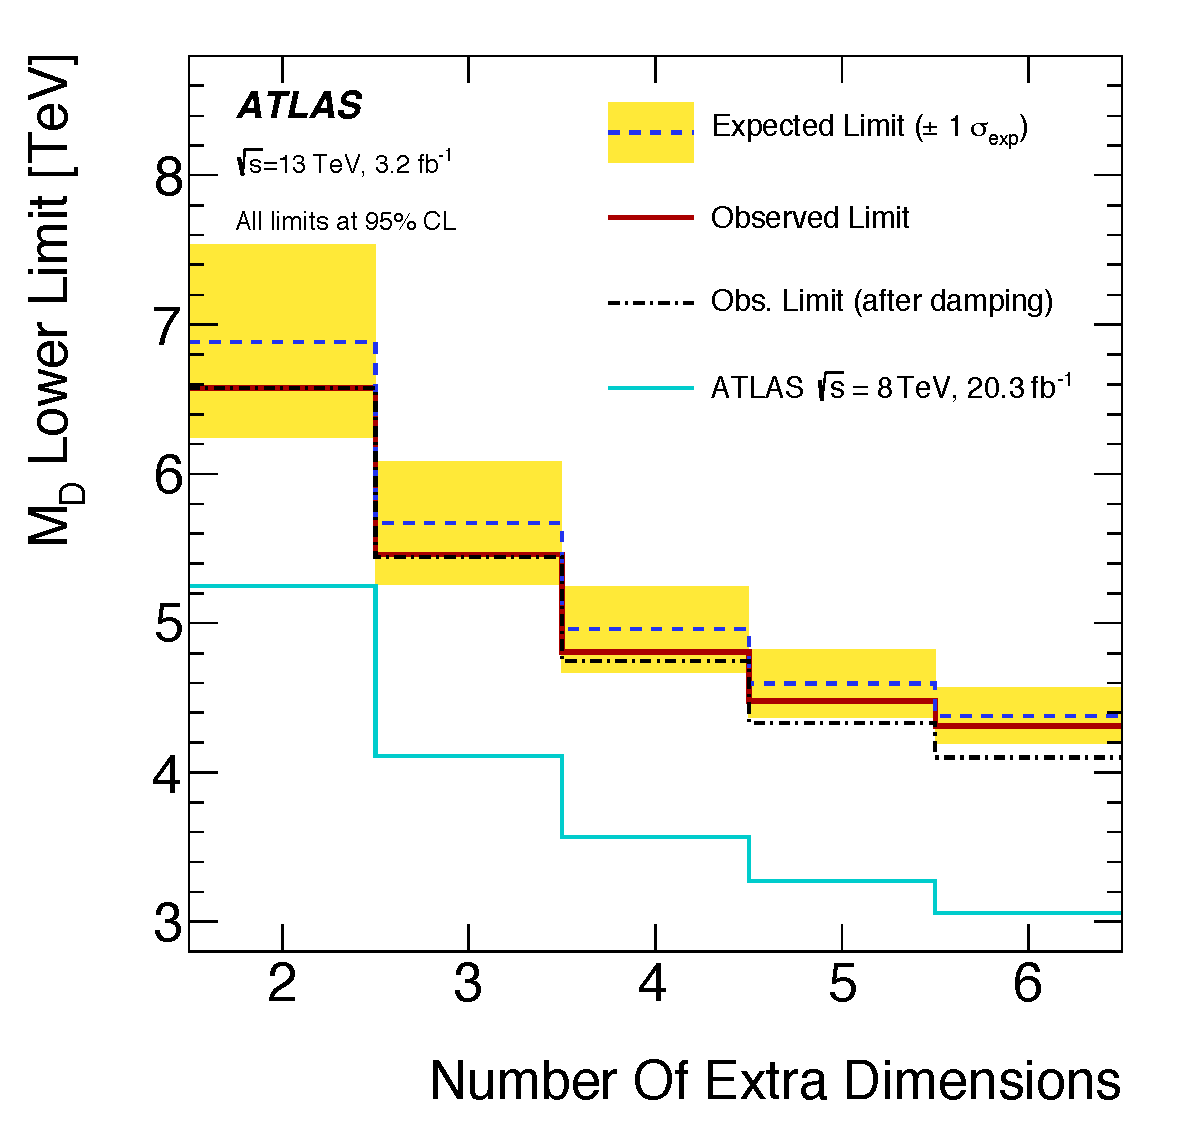
\includegraphics[width=\linewidth]{add_results_2015}
  \caption{Observed and expected lower limits at 95\%~CL on the fundamental
    Planck scale in $4 + n$ dimensions, $\md$, as a function of the number of
    extra dimensions. The dashed blue line is the expected limit using
    3.2~$\ifb$, the yellow band is the $\pm 1 \sigma$ uncertainty on the
    estimate. The black dashed line shows the observed limit after the
    suppression of events with $\hat{s} > \md^2$. Previous result are also
    reported for comparison~\cite{MonoJetPaper}.}
  \label{fig:add_2015}
\end{figure}
%%% Local Variables:
%%% mode: latex
%%% TeX-master: "../search_for_DM_LED_with_ATLAS"
%%% End:
